\documentclass[chaptersright]{informeutn}
\usepackage[utf8]{inputenc}
\usepackage{array}
\usepackage[table]{xcolor}
\usepackage{colortbl}
\usepackage{caption}
\usepackage{graphicx}
\usepackage{amsmath}
\usepackage{multirow}
\usepackage{float}
\usepackage{geometry}[a4paper,margin=2.5cm]
\newcommand{\widemargins}{
  \newgeometry{left=1.5cm,right=1.5cm,top=1.8cm,bottom=1.8cm}
}
\newcommand{\restoremargins}{\restoregeometry}

\materia{Dispositivos Electronicos I}
\titulo{Trabajo Practico N°5: TIRISTORES}
\comision{3R2}
\autores{Documentador y operador: Gaston Grasso 401892\\ Coordinador: Angelo Prieto 401012}
\fecha{4-11-2025}


\begin{document}
\maketitle
\tableofcontents

\chapter{Introduccion}
En este trabajo práctico se analizan distintos dispositivos pertenecientes a la familia de los tiristores: SCR, DIAC y
TRIAC. El objetivo principal es estudiar sus características eléctricas, obtener sus curvas características y comprender
su funcionamiento en distintas condiciones de operación, incluyendo el disparo, la conducción y el apagado.

Las actividades combinan mediciones experimentales en laboratorio con simulaciones, lo que permite observar con precisión
el comportamiento dinámico de cada dispositivo y, al mismo tiempo, contrastarlo con situaciones reales. A través de
estas prácticas, se exploran también algunas aplicaciones típicas de los tiristores, especialmente en el control de
potencia y la conmutación de señales.


\chapter{SCR}
\section{Condición de disparo y corriente de mantenimiento}
\subsection{Actividad de laboratorio}

\begin{figure}[h]
	\centering
	\begin{tikzpicture}
		% Paths, nodes and wires:
		\draw (-6.38, 2) to[american resistor, l={$R_1$}] (-6.38, 4);
		\draw (-6.38, 1) to[american potentiometer] (-6.38, -1);
		\draw (-3.38, -0) to[american resistor, l={$R_G$}] (-5.38, -0);
		\draw (-2.88, -0) to[ammeter, l={$I_G$}] (-0.88, -0);
		\draw (-0.88, -0) to[normal open switch] (1.37, -0);
		\draw (2.154, 2.295) to[empty thyristor, mirror] (2.134, -0.905);
		\draw (2.154, 2.295) to[american resistor, l={$R_2$}] (2.154, 4.295);
		\draw (2.12, -3) to[ammeter, l={$I_{AK}$}] (2.134, -0.905);
		\draw (4.12, -1) to[voltmeter, l={$V_{AK}$}] (4.12, 1);
		\draw (6.12, -1) to[voltmeter, l={$V_{CC}$}] (6.12, 1);
		\draw (4.12, 1) |- (2.12, 2);
		\draw (6.12, 1) |- (2.154, 4.295);
		\draw (4.12, -1) -| (4.12, -3);
		\draw (6.12, -1) -| (6.12, -3);
		\draw (6.12, -3) |- (-6.38, -3);
		\draw (-6.38, -3) -| (-6.38, -1);
		\draw (-6.38, 1) -| (-6.38, 2);
		\draw (2.154, 4.295) |- (2.12, 5);
		\draw (-6.38, 4) -| (-6.38, 5);
		\draw (-5.82, -0) -- (-5.38, -0);
		\draw (-3.13, -3) to[voltmeter, l={$V_G$}] (-3.13, -0);
		\draw (-3.38, -0) -- (-2.88, -0);
		\node[vcc](N1) at (-6.38, 5){} node[anchor=south] at (N1.text){$20V$};
		\node[vcc](N2) at (2.154, 5){} node[anchor=south] at (N2.text){$V_{CC}$};
		\node[ground] at (2.12, -3){};
	\end{tikzpicture}
	\caption{circuito implementado en el laboratorio.}
	\label{fig:circuito-scr}
\end{figure}

Para la realización de la experiencia se siguieron de manera estricta todos los pasos establecidos en las consignas del
trabajo. En primer lugar, se armó el circuito según el esquema provisto y se ajustó la tensión $V_{CC}$ a $0\,\text{V}$.
A continuación, se cerró el circuito en el punto donde se preveía la inclusión del interruptor y se procedió a variar
el potenciómetro para relevar los valores de $V_G$ correspondientes a la tabla \ref{table:ig-vg}

\begin{table}[ht!]
	\centering
	\small
	\begin{tabular}{|c|c|c|c|c|c|c|c|c|c|c|}
		\hline
		$V_G$ [V]  & 0 & 0.057 & 0.116 & 0.18 & 0.238 & 0.302 & 0.393 & 0.485 & 0.543 & 0.611 \\
		\hline
		$I_G$ [mA] & 0 & 0.25  & 0.51  & 0.8  & 1.05  & 1.33  & 1.74  & 2.15  & 2.43  & 2.81  \\
		\hline
	\end{tabular}
	\caption{valores de $I_G = f(V_G)$ obtenidos en laboratorio.}
	\label{table:ig-vg}
\end{table}

\begin{figure}[ht!]
	\centering
	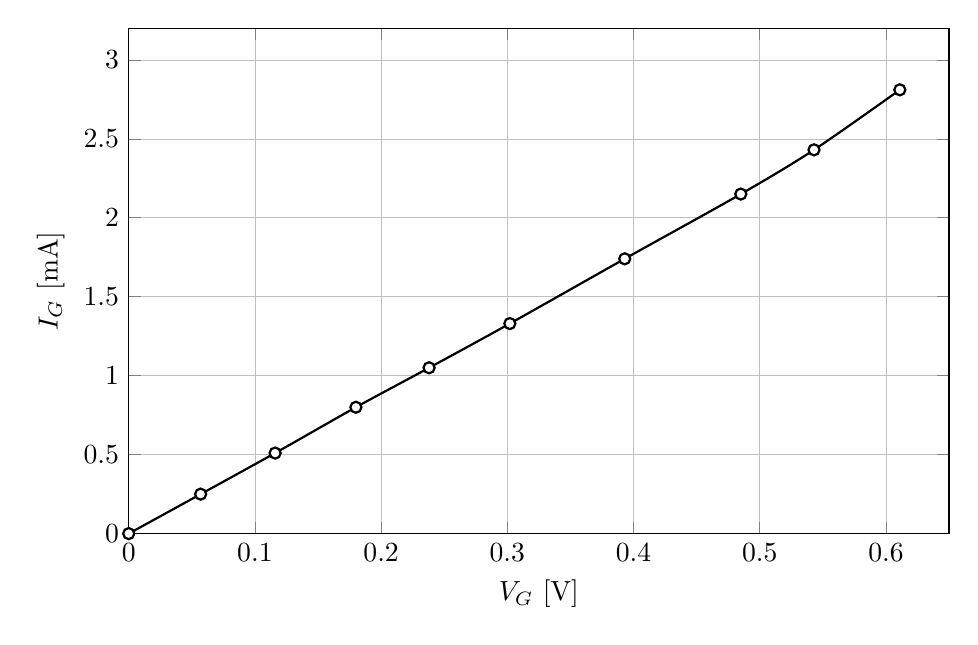
\begin{tikzpicture}
		\begin{axis}[
				width=12cm,
				height=8cm,
				xlabel={$V_G$ [V]},
				ylabel={$I_G$ [mA]},
				grid=both,
				ymin=0, ymax=3.2,
				xmin=0, xmax=0.65,
				major grid style={line width=.2pt,draw=gray!50},
				minor grid style={line width=.1pt,draw=gray!30},
				legend pos=north west
			]

			\addplot[
				thick,
				smooth,
				mark=*,
				mark options={fill=white},
			] coordinates {
					(0,0)
					(0.057,0.25)
					(0.116,0.51)
					(0.18,0.80)
					(0.238,1.05)
					(0.302,1.33)
					(0.393,1.74)
					(0.485,2.15)
					(0.543,2.43)
					(0.611,2.81)
				};

		\end{axis}
	\end{tikzpicture}
	\caption{Curva característica $I_G$ en función de $V_G$.}
	\label{fig:ig-vg}
\end{figure}

Luego, se estableció $V_G = 0\,\text{V}$ con el circuito cerrado y se configuró $V_{CC} = 100\,\text{V}$. A partir de
allí, se incrementó lentamente la tensión de compuerta hasta observar un cambio significativo en la corriente $I_{AK}$,
indicando el disparo del SCR.

Manteniendo el potenciómetro en la posición correspondiente al disparo, se abrió el circuito y se analizó el
comportamiento de la corriente $I_{AK}$. Con el circuito abierto, se disminuyó la tensión $V_{CC}$ en pasos de
$10\,\text{V}$, y en pasos de $1\,\text{V}$ cercano al punto de apagado del SCR, registrando la corriente $I_{AK}$ en
cada caso, que se cuentran en la tabla \ref{table:corriente-mantenimiento}.
Posteriormente, se volvió a aumentar gradualmente $V_{CC}$
hasta alcanzar nuevamente los $100\,\text{V}$, observando la evolución de $I_{AK}$ en este proceso.

\begin{table}[ht!]
	\centering
	\small
	\begin{tabular}{|c|c|c|c|c|c|c|c|c|c|c|c|}
		\hline
		$V_{CC}$ [V]  & 96.6 & 86.6 & 76  & 63.8 & 53  & 45.5 & 43.5  & 41.4  & 39.1  & 37.95 & 36.92 \\
		\hline
		$V_{AK}$ [V]  & 0.7  & 0.7  & 0.7 & 0.7  & 0.7 & 0.71 & 0.716 & 0.723 & 0.742 & 0.757 & 36.92 \\
		\hline
		$I_{AK}$ [mA] & 21   & 20   & 15  & 13   & 9   & 8    & 8     & 8     & 8     & 8     & 0     \\
		\hline
	\end{tabular}
	\caption{valores de obtenidos en laboratorio.}
	\label{table:corriente-mantenimiento}
\end{table}


Con la tensión restituida a $100\,\text{V}$, se cerró nuevamente el circuito verificando que los valores de $V_G$ e $I_G$
coincidieran con los obtenidos previamente. Se analizó el comportamiento de $I_{AK}$ al cerrar el circuito y, luego,
se abrió nuevamente para observar la variación correspondiente en la corriente.

Finalmente, se desconectaron las alimentaciones sin modificar la posición del potenciómetro y se invirtieron las
conexiones del ánodo y cátodo del SCR. Se reconectaron las fuentes, se cerró el circuito y se estudió el
comportamiento de $I_{AK}$ bajo esta nueva configuración.

La alternativa planteada para disparar el SCR implica la aplicación de una corriente $I_G$ en la compurta del dispositivo.
Esto dispara el dispositivo ya que la aplicación de esta corriente reduce la tensión de ruptura, tensión a la cual se
dispara el dispositivo. Otra forma de disparar el SCR sin corriente en la compuerta, es alcanzando la tensión de ruptura
para $I_G = 0$, tensión que es muy alta (mayor a 600V para el dispositivo que utilizamos).

\begin{figure}[H]
	\centering
	\includegraphics[width=.95\linewidth]{Images/circuito SCR armado.jpeg}
	\caption{Circuito para experimentacion armado utilizando un paralelo de 6 resistencias de potencia.}
\end{figure}

\subsection{Actividad de simulación}


\subsection*{1) Montaje}
Se armó el circuito indicado con \(\text{R1}=\text{R2}=4{,}7~\text{k}\Omega\).
Nodos: \(\,V_g\) (compuerta), \(\,V_a\) (ánodo), \(\,V_k\) (cátodo = 0~V).

\subsection*{2–4) \(V_2=0\) y barrido de \(V_1\) — Curva \(I_G=f(V_G)\)}
Directiva: \verb|.dc V1 0 0.7 0.01| \;(\(0\to0{,}7\) V, paso 10 mV).
Se graficó \(I_G=I(U2:G)\) vs. \(V_G=V(V_g)-V(V_k)\).

\begin{figure}[H]
	\centering
	\includegraphics[width=\linewidth]{Images/Simulacion 1.1.png}
	\caption{\(I_G\)–\(V_G\) con \(V_2=0\) V.}
\end{figure}

\textbf{Lectura:} curva con umbral alrededor de \(0{,}55{-}0{,}65\) V y crecimiento
exponencial; coincide con la \(I\)-\(V\) de una unión \(p\!-\!n\) directa (igual forma que un
diodo o \(I_B\)–\(V_{BE}\) de un BJT). Para \(V_G=0{,}70\) V se observa \(I_G\approx 4\) mA.

\subsection*{5–6) Disparo por sobretensión con compuerta abierta \((I_G=0)\)}
Se abre compuerta (sin excitación en \(V_1\)) y se barre \(V_2\):
\verb|.dc V2 0 800 10|.
Se grafica \(I_A=I(U2:A)\) en función de \(V_{AK}=V(V_a)-V(V_k)\).

\begin{figure}[H]
	\centering
	\includegraphics[width=\linewidth]{Images/Simulacion 1.2.png}
	\caption{\(I_A=f(V_{AK})\) con \(I_G=0\) (breakover).}
\end{figure}

\textbf{Lectura:} corriente de fuga baja hasta alcanzar el \emph{breakover};
en el modelo usado ocurre cerca de \(V_{BO}\approx 6\times10^2\) V.
Luego aparece la región de resistencia diferencial negativa y el enclavamiento:
el SCR queda en conducción hasta que \(I_A<I_H\).

\subsection*{7) Disparo por compuerta a \(V_2=100\) V}
Se fija \(V_2=100\) V y se barre \(V_1\): \verb|.dc V1 0 20 0.01|.
Se monitorea el salto de \(I_A\) para detectar el disparo controlado por compuerta.

\begin{figure}[H]
	\centering
	\includegraphics[width=\linewidth]{Images/Simulacion 1.3.png}
	\caption{\(V_2=100\) V. Barrido de \(V_1\) y cambio brusco de \(I_A\) (disparo).}
\end{figure}

\textbf{Lectura y estimación:} el disparo ocurre a
\(V_{1,\text{trig}}\approx 9{,}8{-}10\) V.
Aproximando \(V_{GK(\text{ON})}\simeq 0{,}6\) V:
\[
	I_{G,\text{trig}}\;\approx\;\frac{V_{1,\text{trig}}-0{,}6}{4{,}7~\text{k}\Omega}
	\;\approx\;2~\text{mA}.
\]
Tras el disparo, \(I_A\) queda fijada por \(V_2\) y \(R_2\) (enclavamiento).

\begin{itemize}
	\item \(I_G\!-\!V_G\): misma forma que un diodo; umbral \(\sim 0{,}6\) V.
	\item Con \(I_G=0\): disparo por \emph{breakover} a \(V_{BO}\sim 600\) V y enclavamiento.
	\item Con \(V_2=100\) V: disparo por compuerta con \(I_{G,\text{trig}}\) del orden de mA.
\end{itemize}



\section{Obtención de curva característica}
Con la experiencia de la actividad anterior, se buscará controlar el disparo del SCR
mediante diferentes corrientes IG. Además, se identificará si efectivamente la conmutación de
inactivo a activo se da a diferentes valores de $V_{AK}$.

\subsection{Actividad de laboratorio}
Para la realización de la actividad se siguieron los pasos detallados en la guía de trabajo. En primer lugar, se armó
el circuito de la Fig. \ref{fig:circuito-scr}.

A continuación, se completaron los valores de la tabla \ref{table:disparo} fijando el valor de $I_G$ y variando la
tensión $V_{CC}$ hasta observar el disparo del SCR. Para cada caso se relevaron los valores de
$V_{CC}$, $I_{AK}$ y $V_{AK}$ correspondientes al punto de disparo.

\begin{table}[ht!]
	\centering
	\small
	\begin{tabular}{|c|c|c|c|}
		\hline
		$I_G$ [mA] & $V_{CC}$ [V] & $I_{AK}$ [mA] & $V_{AK}$ [V] \\
		\hline
		2.92       & 600          & 127.51        & 0.7          \\
		2.96       & 465          & 98.79         & 0.7          \\
		2.98       & 398          & 84.53         & 0.7          \\
		3.00       & 345          & 73.25         & 0.7          \\
		3.02       & 295          & 62.62         & 0.7          \\
		\hline
	\end{tabular}
	\caption{relevamiento de disparo del SCR para diferentes valores de $I_G$.}
	\label{table:disparo}
\end{table}

Posteriormente, se procedió a completar los valores de la \ref{table:curva-scr}, nuevamente fijando el valor de $I_G$ y variando
$V_{CC}$. En cada caso se registraron los valores de $I_{AK}$ y $V_{AK}$.
Se tuvo en cuenta ajustar los valores de corrientes y tensiones según las características del dispositivo utilizado. Esto
se hace con el objetivo de obtener la curva característica del dispositivo, la cual se grafíca en la figura \ref{fig:curva-scr}.

\begin{table}[h]
	\centering
	\resizebox{0.9\textwidth}{!}{
		\begin{tabular}{|cc|cc|cc|cc|cc|}
			\hline
			\multicolumn{2}{|c|}{$I_{G} = 2.92mA\,$}
			             & \multicolumn{2}{c|}{$I_{G} = 2.96mA\,$}
			             & \multicolumn{2}{c|}{$I_{G} = 2.98mA\,$}
			             & \multicolumn{2}{c|}{$I_{G} = 3.00mA\,$}
			             & \multicolumn{2}{c|}{$I_{G} = 3.02mA\,$}                                                                                                                             \\
			\hline
			$V_{AK}$ [V] & $I_{AK}$ [mA]                           & $V_{AK}$ [V] & $I_{AK}$ [mA] & $V_{AK}$ [V] & $I_{AK}$ [mA] & $V_{AK}$ [V] & $I_{AK}$ [mA] & $V_{AK}$ [V] & $I_{AK}$ [mA] \\
			\hline
			0            & 0.000                                   & 0            & 0.000         & 0            & 0.000         & 0            & 0.000         & 0            & 0.000         \\
			50           & 0.000                                   & 50           & 0.000         & 50           & 0.000         & 50           & 0.000         & 50           & 0.000         \\
			100          & 0.000                                   & 98           & 0.000         & 100          & 0.000         & 100          & 0.000         & 98.3         & 0.000         \\
			200          & 0.000                                   & 148          & 0.000         & 147.5        & 0.000         & 148.2        & 0.000         & 148          & 0.000         \\
			300          & 0.000                                   & 197.5        & 0.000         & 198          & 0.000         & 200          & 0.000         & 200          & 0.000         \\
			350          & 0.000                                   & 247.5        & 0.000         & 250          & 0.000         & 247          & 0.000         & 247.5        & 0.638         \\
			400          & 0.000                                   & 296.1        & 0.000         & 296.3        & 0.000         & 297          & 0.000         & 297.5        & 0.53          \\
			450          & 0.000                                   & 343.5        & 0.000         & 346          & 0.000         & 320.8        & 0.89          & 0.7          & 62.62         \\
			500          & 0.000                                   & 392.4        & 0.000         & 0.7          & 84.53         & 0.7          & 73.25         & -            & -             \\
			550          & 0.000                                   & 443.6        & 0.000         & -            & -             & -            & -             & -            & -             \\
			600          & 0.000                                   & 0.7          & 98.79         & -            & -             & -            & -             & -            & -             \\
			0.7          & 127.51                                  & -            & -             & -            & -             & -            & -             & -            & -             \\
			\hline
		\end{tabular}
	}
	\caption{Tabla de $I_{AK} = f(V_{AK})$ para distintos valores de $I_{G}$.}
	\label{table:curva-scr}
\end{table}

\begin{figure}[ht]
	\centering
	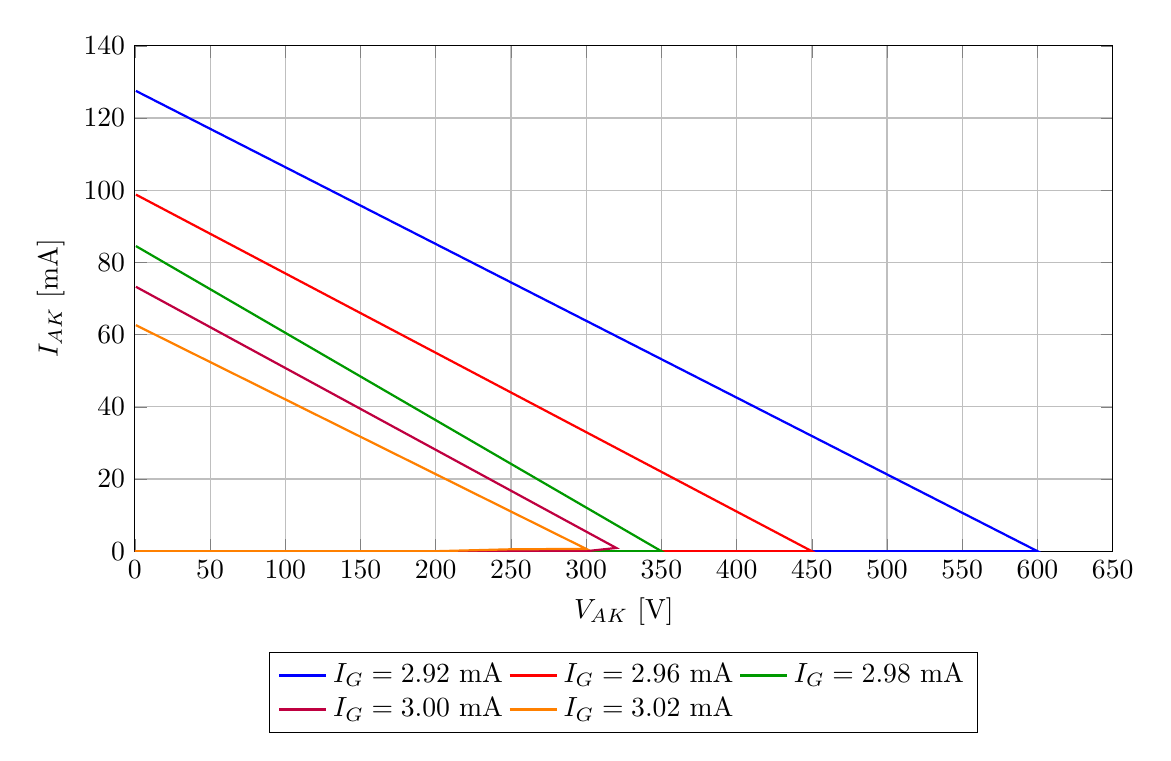
\begin{tikzpicture}
		\begin{axis}[
				width=14cm,
				height=8cm,
				xlabel={$V_{AK}$ [V]},
				ylabel={$I_{AK}$ [mA]},
				grid=both,
				ymin=0, ymax=140,
				xmin=0, xmax=650,
				legend style={at={(0.5,-0.2)},anchor=north,legend columns=3},
			]

			% ---- IG = 2.92 mA ----
			\addplot[blue, thick] coordinates {
					(0,0) (50,0) (100,0) (200,0) (300,0) (400,0) (500,0) (600,0)
					(0.7,127.51)
				};
			\addlegendentry{$I_G = 2.92$ mA}

			% ---- IG = 2.96 mA ----
			\addplot[red, thick] coordinates {
					(0,0) (50,0) (100,0) (150,0) (200,0) (250,0) (300,0)
					(350,0) (400,0) (450,0) (0.7, 98.79)
				};
			\addlegendentry{$I_G = 2.96$ mA}

			% ---- IG = 2.98 mA ----
			\addplot[green!60!black, thick] coordinates {
					(0,0) (50,0) (100,0) (150,0) (200,0) (250,0) (300,0) (350,0) (0.7,84.53)
				};
			\addlegendentry{$I_G = 2.98$ mA}

			% ---- IG = 3.00 mA ----
			\addplot[purple, thick] coordinates {
					(0,0) (50,0) (100,0) (150,0) (200,0) (250,0) (300,0) (320,0.9)
					(0.7,73.25)
				};
			\addlegendentry{$I_G = 3.00$ mA}

			% ---- IG = 3.02 mA ----
			\addplot[orange, thick] coordinates {
					(0,0) (50,0) (100,0) (150,0) (200,0) (250,0.53) (300,0.638)
					(0.7,62.62)
				};
			\addlegendentry{$I_G = 3.02$ mA}

		\end{axis}
	\end{tikzpicture}
	\caption{Curvas características $I_{AK}(V_{AK})$ del SCR para distintos $I_G$.}
	\label{fig:curva-scr}
\end{figure}

Con estos resultados se puede demostrar lo afirmado en el ejercicio anterior, que la tensión de ruptura o disparo del
SCR disminuye con la aplicación de una corriente en la compuerta del dispositivo. Además, la curva característica
obtenida se asemeja a lo estudiado en la teoría.
\vspace{10cm}


\clearpage
\section{Funcionamiento con corriente alterna}
En esta actividad se estudian dos aspectos fundamentales del funcionamiento del SCR: el control de disparo y el proceso
de apagado. Estas características resultan esenciales en aplicaciones donde es necesario regular la transferencia de
potencia hacia una carga a partir de una fuente de corriente alterna.

La experiencia se desarrolla íntegramente en un entorno de simulación, lo cual ofrece ventajas significativas respecto
de una práctica de laboratorio convencional. La simulación permite visualizar con mayor detalle las formas de onda
involucradas y facilita la realización de múltiples ensayos modificando parámetros como la tensión de alimentación o
el valor de componentes específicos. Gracias a ello, es posible analizar con mayor precisión el comportamiento del
dispositivo y comprender de manera más completa su dinámica de conducción y bloqueo.
\subsection{Actividad de simulación}


\subsubsection*{2) Señales observadas \(\,V_{in},\,V_{R3}\, e\, I_G\)}
En la simulación se cruzaron en una misma gráfica:
tensión de entrada \(V_{in}\), caída en la carga \(V_{R3}\) y corriente de compuerta \(I_G\).
El barrido por \verb|.STEP| genera familias de curvas para distintas posiciones del
potenciómetro.

\begin{figure}[H]
	\centering
	\includegraphics[width=.95\linewidth]{Images/Simulacion 2.1.png}
	\caption{Resultados: \(V_{in}\) (verde), \(V_{R3}\) (azul) e \(I_G\) (rojo) para varios \(p\).}
\end{figure}

\subsubsection*{3) Variación del parámetro \(p\) (\texttt{.STEP})}
Al aumentar \(p\) crece la constante de tiempo \(R_2C_1\) y el pulso de \(I_G\) se retrasa,
incrementando el ángulo de disparo \(\alpha\) y reduciendo el valor eficaz en la carga.
Para \(p\) pequeño, \(I_G\) aparece temprano (menor \(\alpha\)) y la potencia transferida es mayor.

\subsection*{4a) Explicación de funcionamiento y rol del capacitor}
El lazo \(R_1\!-\!R_2\!-\!C_1\) genera un desfase y conforma un pulso en la compuerta a
cada semiciclo positivo de \(V_{in}\) (a través de \(R_3\) y \(D_1\)).
Cuando \(V_{GK}\) supera el umbral y \(I_G \ge I_{G,\text{trig}}\), el SCR conmuta y
\(V_{R3}\) replica el semiciclo restante de \(V_{in}\) hasta el cruce por cero.
El capacitor \(C_1\) es clave: fija la constante de tiempo con \(R_2\) para mover \(\alpha\),
y además proporciona un pulso de compuerta bien definido (limitando corriente
continua por la unión \(G\!-\!K\) y mejorando la inmunidad a ruidos).

\subsubsection*{4b) Corrientes en disparo y apagado}
\textbf{En el disparo.}
De la familia de curvas rojas (\(I_G\)) se mide el pico en el instante en que
\(V_{R3}\) sube abruptamente. En la simulación, según \(p\),
\[
	I_{G,\text{trig}} \approx 0{,}5~\text{mA} \; \text{a} \; 4{,}5~\text{mA},
\]
coherente con un SCR sensible (mA).

\textbf{En el apagado.}
Con carga resistiva pura, el apagado ocurre por cruce por cero de la corriente;
por lo tanto la corriente de ánodo–cátodo en el instante de apagado verifica
\[
	I_{AK}(t_{\text{off}})\approx 0~\text{A}\ (< I_H),
\]
lo cual coincide con lo esperado teóricamente: el enclavamiento se pierde
cuando \(I_{AK}<I_H\) y, con \(R\) puro, eso sucede exactamente en el cruce por cero.

\subsubsection*{4c) Ángulo mínimo y máximo controlable (\(\alpha\))}
Se midió el retardo desde el cruce por cero de \(V_{in}\) hasta el frente de subida
de \(V_{R3}\) en cada semiciclo y se convirtió a grados mediante
\[
	\alpha \,[^\circ] \;=\; 180^\circ \,\frac{t_d}{T/2}\,,
	\qquad T=20~\text{ms} \text{ (50 Hz)}.
\]
De la simulación:
\[
	\alpha_{\min}\approx 25^\circ \ \ (\;p \simeq 0{,}1~\text{k}\Omega\;),\qquad
	\alpha_{\max}\approx 155^\circ \ \ (\;p \simeq 4{,}9~\text{k}\Omega\;).
\]
Los límites no llegan exactamente a \(0^\circ/180^\circ\) por el umbral \(V_{GK}\),
la corriente de disparo requerida y el recorte del circuito de compuerta.

\subsubsection*{Notas de implementación}
Para reproducibilidad, medir \(\alpha\) con cursores sobre \(V_{in}\) y \(V_{R3}\),
y calcular \(I_G\) con \verb|I(U1:G)|. En LTspice, activar \emph{Add Trace} y
graficar por paso (\emph{Plot Settings} \(\rightarrow\) \emph{Add Trace} \(\rightarrow\)
\emph{Function: last/first}) para leer \(\alpha_{\min}\) y \(\alpha_{\max}\) por cada \(p\).



\chapter{DIAC}
Objetivo: determinar la polarización y funcionamiento del DIAC.
\section{Actividad de laboratorio}

Para la realización de la actividad se siguieron los pasos establecidos. En primer lugar, se armó el circuito de la figura \ref{fig:circuito-diac}
seleccionando un valor de resistencia de $4.7K \Omega$, suficiente de acuerdo con la información provista en el datasheet del DIAC.

\begin{figure}[ht!]
	\centering
	\begin{tikzpicture}
		% Paths, nodes and wires:
		\draw (-1.75, -1) to[full bidirectionaldiode] (-1.75, 1);
		\draw (1.25, -1) to[voltmeter, l={$V_2$}] (1.25, 1);
		\draw (-1.75, 1) to[american resistor, l={$R$}] (-1.75, 3);
		\node[vcc](N1) at (-1.75, 3.5){} node[anchor=south] at (N1.text){$V_{CC}$};
		\draw (-1.75, 1) -- (1.25, 1);
		\draw (-1.75, -1) -- (1.25, -1);
		\draw (3.25, -0) to[voltmeter, l={$V_1$}] (3.25, 2);
		\draw (-1.75, 3) -| (3.25, 2);
		\draw (-1.75, -3) to[ammeter] (-1.75, -1);
		\node[ground] at (-1.75, -3){};
		\draw (-1.75, 3) -| (-1.75, 3.5);
		\draw (3.25, -0) |- (-1.75, -1.25);
	\end{tikzpicture}
	\caption{circuito implementado en el laboratorio.}
	\label{fig:circuito-diac}
\end{figure}

A continuación, se varió la tensión alimentación $V_{CC}$ desde $0\,\text{V}$ hasta $50\,\text{V}$ siguiendo los valores
indicados en la tabla correspondiente. Para cada caso se midieron la corriente circulante y la caída de tensión en el DIAC.

Luego, se invirtieron los terminales del DIAC y se repitieron las variaciones y mediciones detalladas en los pasos anteriores.

En la tabla \ref{table:diac} se puede observar los valores obtenidos, que son los mismos para las dos polarizades del
DIAC. En la figura \ref{fig:diac} se grafican dichos valores.

\begin{table}[ht!]
	\centering
	\small
	\begin{tabular}{|c|c|c|c|c|c|c|c|c|c|}
		\hline
		$V_{CC}$ [V]  & 0 & 10 & 20 & 30 & 32   & 34   & 40   & 45   & 50   \\
		\hline
		$V_{AK}$ [V]  & 0 & 10 & 20 & 30 & 23.8 & 23.4 & 22.6 & 22.2 & 21.9 \\
		\hline
		$I_{AK}$ [mA] & 0 & 0  & 0  & 0  & 1.74 & 2.24 & 3.72 & 4.9  & 5.92 \\
		\hline
	\end{tabular}
	\caption{relevamiento de disparo del SCR para diferentes valores de $I_G$.}
	\label{table:diac}
\end{table}

\begin{figure}[ht!]
	\centering
	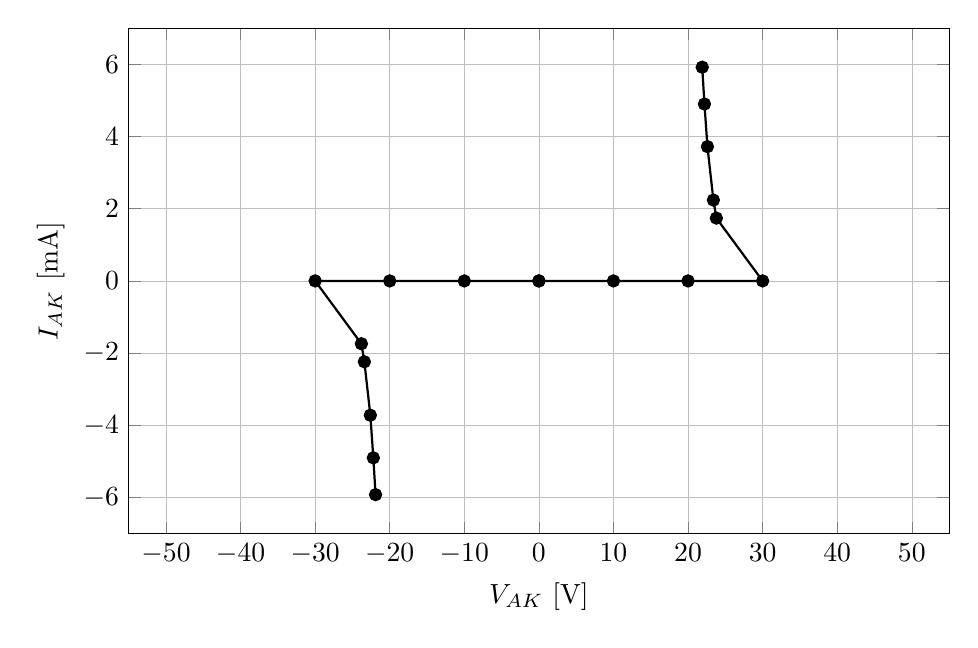
\begin{tikzpicture}
		\begin{axis}[
				width=12cm, height=8cm,
				xlabel={$V_{AK}$ [V]},
				ylabel={$I_{AK}$ [mA]},
				xmin=-55, xmax=55,
				ymin=-7, ymax=7,
				grid=both,
				grid style={line width=.1pt, draw=gray!30},
				major grid style={line width=.2pt,draw=gray!50},
				legend pos=north west,
				enlargelimits=false,
				clip=false,
			]

			% ----------- Curva positiva -----------
			\addplot[
				mark=*,
				mark options={fill=white},
				thick,
			] coordinates {
					(0,0)
					(10,0)
					(20,0)
					(30,0)
					(23.8,1.74)
					(23.4,2.24)
					(22.6,3.72)
					(22.2,4.90)
					(21.9,5.92)
				};

			% ----------- Curva negativa (reflejada) -----------
			\addplot[
				mark=*,
				mark options={fill=white},
				thick,
			] coordinates {
					(0,0)
					(-10,0)
					(-20,0)
					(-30,0)
					(-23.8,-1.74)
					(-23.4,-2.24)
					(-22.6,-3.72)
					(-22.2,-4.90)
					(-21.9,-5.92)
				};

			% ----------- Puntos experimentales ----------
			\addplot[only marks, mark=*, mark size=2pt] coordinates {
					(0,0) (10,0) (20,0) (21.9,5.92)
					(22.2,4.90) (22.6,3.72) (23.4,2.24) (23.8,1.74) (30,0)

					(0,0) (-10,0) (-20,0) (-21.9,-5.92)
					(-22.2,-4.90) (-22.6,-3.72) (-23.4,-2.24) (-23.8,-1.74) (-30,0)
				};

		\end{axis}
	\end{tikzpicture}
	\caption{curva $I_{AK}=f(V_{AK})$ del DIAC.}
	\label{fig:diac}
\end{figure}
\clearpage
\chapter{TRIAC}
\section{Polarización y funcionamiento}
\begin{figure}[ht]
	\centering
	\resizebox{0.5\textwidth}{!}{
		\begin{tikzpicture}
			% Paths, nodes and wires:
			\draw (0.02, 2) to[american resistor, l={$R$}] (0.02, 4);
			\node[ground] at (0.02, -3.7){};
			\draw (-1.253, -0.018) to[full bidirectionaldiode] (-3.253, -0.018);
			\draw (0, -1.75) to[full triac] (0.02, 0.3);
			\draw (-5, -0) to[ammeter, l={$I_G$}] (-3.5, -0);
			\draw (-6, -1) to[american potentiometer, mirror] (-6, 1);
			\draw (0.02, 0.3) |- (0, 2);
			\draw (-6, 1) -- (-6, 2) -- (0, 2);
			\draw (0.02, -3.7) to[ammeter, l={$I_A$}] (0, -1.75);
			\draw (2.25, -2) to[voltmeter, l={$V_{CC}$}] (2.25, 1);
			\draw (2.25, -2) |- (0.02, -3.7);
			\draw (2.25, 1) |- (0.02, 4);
			\draw (-6, -1) |- (0.02, -3.7);
			\node[vcc] at (0, 4){};
			\node[vcc](N1) at (0.02, 4){} node[anchor=south] at (N1.text){$V_{CC}$};
			\draw (-5, -0) -- (-5.44, -0);
			\draw (-3.25, -0) -- (-3.5, -0);
			\draw (-1.253, -0.018) -- (-0.753, -0.018);
		\end{tikzpicture}
	}
	\caption{circuito implementado en el laboratorio.}
\end{figure}


\begin{figure}[H]
	\centering
	\includegraphics[width=.5\linewidth]{Images/Circuito armado Triac.jpeg}
	\caption{Circuito implementado en una protoboard.}
\end{figure}


\newcommand{\VCCA}{80}
\newcommand{\VCCB}{130}
\newcommand{\VCCC}{180}

\begin{table}[H]
	\centering
	\setlength{\tabcolsep}{5pt}
	\renewcommand{\arraystretch}{1.12}
	\rowcolors{2}{black!3}{white}
	\begin{tabular}{
		c|*{2}{>{\centering\arraybackslash}p{1.6cm}}|
		*{2}{>{\centering\arraybackslash}p{1.6cm}}|
		*{2}{>{\centering\arraybackslash}p{1.6cm}}}
		\rowcolor{black!8}
		\multicolumn{1}{c|}{$V_1$ [V]}        &
		\multicolumn{2}{c|}{$V_{CC}=\VCCA$ V} &
		\multicolumn{2}{c|}{$V_{CC}=\VCCB$ V} &
		\multicolumn{2}{c}{$V_{CC}=\VCCC$ V}                                                                                            \\
		\rowcolor{black!8}
		                                      & $I_G$ [$\mu$A] & $I_A$ [mA] & $I_G$ [$\mu$A] & $I_A$ [mA] & $I_G$ [$\mu$A] & $I_A$ [mA] \\
		\hline
		0                                     & 0              & 0          & 0              & 0          & 0              & 0          \\
		5                                     & 0              & 0          & 0              & 0          & 0              & 0          \\
		10                                    & 0              & 0          & 0              & 0          & 0              & 0          \\
		15                                    & 0              & 0          & 0              & 0          & 0              & 0          \\
		20                                    & 0              & 0          & 0              & 0          & 0              & 0          \\
		25                                    & 0              & 0          & 0              & 0          & 0              & 0          \\
		30                                    & 0              & 0          & 0              & 0          & 0              & 0          \\
		31                                    & 0              & 0          & 0              & 0          & 0              & 0          \\
		31.6                                  &                &            & 4.53           & 4.57       &                &            \\
		32                                    & 3.4            & 3.4        &                &            & 0              & 37.1       \\
		33.0                                  & 3.8            & 3.9        &                &            &                &            \\
		33.1                                  & 4.15           & 4.15       &                &            &                &            \\
		33.2                                  & 4.6            & 4.8        &                &            &                &            \\
		33.3                                  & 4.7            & 6.2        &                &            &                &            \\
		23.4                                  &                &            & 4.53           & 4.57       &                &            \\
		23.3                                  & 3.8            & 3.9        &                &            &                &            \\
		23.1                                  & 4.15           & 4.15       &                &            &                &            \\
		23.2                                  & 4.6            & 4.8        &                &            &                &            \\
		23.7                                  & 4.3            & 6.0        &                &            &                &            \\
		0.3                                   &                &            & 0              & 26.7       &                &            \\
		50                                    &                &            &                &            & 0              & 0          \\
		0                                     & 0              & 16.3       &                &            &                &            \\
	\end{tabular}
	\caption{Relevamiento de puntos para el trazado de $I_A=f(I_G)$ con tres valores de $V_{CC}$.}
\end{table}

% ===================== GRÁFICO IA = f(IG) EN EL MISMO EJE ===================
% Cargamos exactamente los pares (IG, IA) medidos para cada VCC.
\begin{figure}[H]
	\centering
	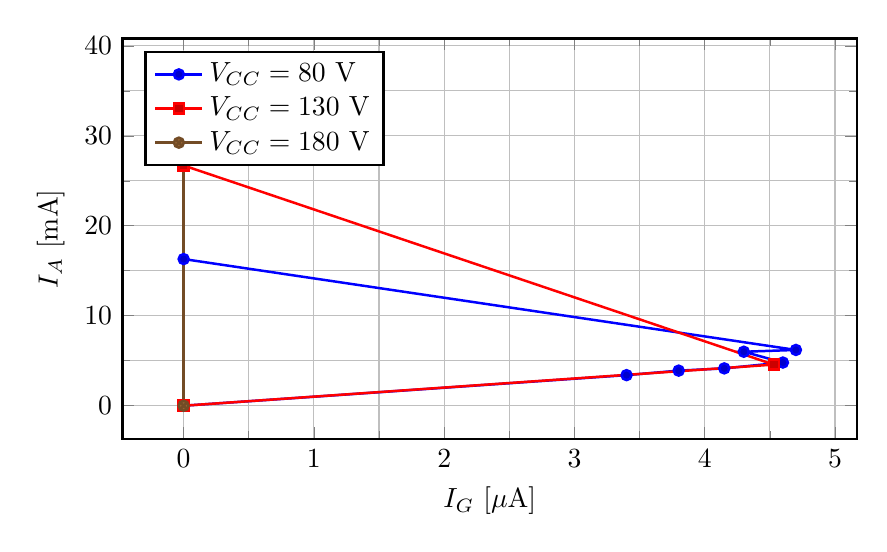
\begin{tikzpicture}
		\begin{axis}[
				width=0.9\linewidth, height=0.55\linewidth,
				xlabel={$I_G$ [$\mu$A]}, ylabel={$I_A$ [mA]},
				grid=both, minor tick num=1,
				legend pos=north west, legend cell align=left,
				line width=0.9pt, mark=*, mark size=1.8pt,
			]
			% ---- VCC = 80 V ----------------------------------------------------------
			\addplot+ coordinates {
					(0,0)
					(3.4,3.4)
					(3.8,3.9)
					(4.15,4.15)
					(4.6,4.8)
					(4.3,6.0)
					(4.7,6.2)
					(0,16.3) % punto de mantenimiento/latch observado
				};
			\addlegendentry{$V_{CC}=80$ V}

			% ---- VCC = 130 V ---------------------------------------------------------
			\addplot+ coordinates {
					(0,0)
					(4.53,4.57)
					(4.53,4.57) % repetido porque aparece en dos V1 distintos
					(0,26.7)
				};
			\addlegendentry{$V_{CC}=130$ V}

			% ---- VCC = 180 V ---------------------------------------------------------
			\addplot+ coordinates {
					(0,0)
					(0,37.1)
				};
			\addlegendentry{$V_{CC}=180$ V}
		\end{axis}
	\end{tikzpicture}
	\caption{Curvas características $I_A=f(I_G)$ para $V_{CC}\in\{80,130,180\}\,\mathrm{V}$.}
\end{figure}

% =============================== CONCLUSIONES ===============================
\noindent\textbf{Conclusiones.}
Las curvas $I_A=f(I_G)$ muestran un umbral de disparo $I_{G,\text{th}}$: por debajo de ese valor
la conducción es nula; superado, $I_A$ crece con alta pendiente (modo de disparo/latch).
Con mayor $V_{CC}$, el dispositivo sostiene corrientes de ánodo más grandes para valores similares
de $I_G$, y el mantenimiento de conducción (holding) aparece a corrientes mayores. Los puntos
$(I_G{=}0,\ I_A{>}0)$ registrados en $V_{CC}=80$ y $180~\mathrm{V}$ evidencian el estado
mantenido tras el disparo. La región cercana al umbral presenta mayor dispersión, esperable por
tolerancias y efectos térmicos. En síntesis, los datos son consistentes con el mecanismo de disparo
y su dependencia con la tensión de alimentación.














\section{Aplicación: control de disparo (Dimmer)}

\subsection{Actividad de laboratorio}

\begin{enumerate}
	\item Se conectó el transformador de aislamiento a la red eléctrica y luego el
	      osciloscopio a la salida del transformador. Esto permitió aislar galvánicamente el
	      instrumento del circuito dimmer, evitando cruces de potencial con la línea.
	\item Se llevó el potenciómetro al valor óhmico máximo.
	\item Se observó la forma de onda en el osciloscopio y se graficó la tensión sobre la
	      carga resistiva (lámpara incandescente de 20 W).
	\item Se variaron las posiciones del potenciómetro registrando tres oscilogramas
	      representativos: resistencia máxima, intermedia y mínima.
	\item Finalmente, se estimó la corriente de mantenimiento $I_H$ del TRIAC mediante un método
	      indirecto, a partir de la tensión de red y la resistencia equivalente de la lámpara.
\end{enumerate}

\subsection{Análisis de las gráficas relevadas}

En el dimmer con DIAC–TRIAC, el ángulo de disparo $\alpha$ está determinado por la constante de
tiempo $RC$ del circuito de compuerta. Al aumentar el valor del potenciómetro, crece
$\tau=RC$ y la tensión del capacitor tarda más en alcanzar el \emph{breakover} del DIAC
($\approx30$ V), por lo que $\alpha$ aumenta y la potencia en la carga disminuye.

De las tres capturas obtenidas:

\begin{itemize}
	\item \textbf{Potenciómetro al máximo (mayor $R$):}
	      La conducción inicia tarde en cada semiciclo ($\alpha$ grande), y se observa un recorte
	      pronunciado al comienzo de cada semiciclo. La potencia disipada en la carga es baja.\\[4pt]
	      \begin{center}
		      \includegraphics[width=0.6\textwidth]{Images/potenciometro al maximo Dimmer.jpeg}
	      \end{center}

	\item \textbf{Posición intermedia:}
	      $\alpha$ medio. El intervalo de conducción crece y la tensión eficaz en la carga
	      aumenta. Se mantiene la simetría entre semiciclos, lo que indica un disparo parejo por
	      el DIAC.\\[4pt]
	      \begin{center}
		      \includegraphics[width=0.6\textwidth]{Images/Potenciometro a la mitad Dimmer.jpeg}
	      \end{center}

	\item \textbf{Potenciómetro al mínimo (menor $R$):}
	      $\alpha$ pequeño. El TRIAC conduce casi todo el semiciclo y la tensión eficaz sobre la
	      carga se aproxima a la de la red. La lámpara ilumina con máxima intensidad.\\[4pt]
	      \begin{center}
		      \includegraphics[width=0.6\textwidth]{Images/potenciometro al minimo Dimmer.jpeg}
	      \end{center}
\end{itemize}

En los tres casos se observa que el TRIAC se apaga en las proximidades del cruce por cero, lo
que corresponde al instante donde la corriente de carga cae por debajo de la corriente de
mantenimiento $I_H$.

\subsection{Medición indirecta de la corriente de mantenimiento $I_H$}

Para estimar $I_H$, se consideró que la lámpara de 20 W a 220 V presenta una resistencia media:
\[
	R_L = \frac{V_\mathrm{RMS}^2}{P} = \frac{220^2}{20} \approx 2420~\Omega.
\]
La tensión de pico de la red es $V_m = 311$ V, por lo tanto:
\[
	I_\mathrm{max} = \frac{V_m}{R_L} \approx 0.128~\text{A}.
\]

A partir de las oscilografías, el apagado se produce muy próximo al cruce por cero,
correspondiente a $\beta \approx 175^{\circ}$. Sustituyendo en:
\[
	I_H = \frac{V_m}{R_L}\sin(\beta),
\]
se obtiene:
\[
	I_H = 0.128\,\sin(175^{\circ}) \approx 0.011~\text{A}.
\]

Por lo tanto, la corriente de mantenimiento estimada es aproximadamente:
\[
	I_H \approx 11~\text{mA},
\]
valor coherente con los TRIACs de uso general (TIC-226, BT136, etc.), que presentan $I_H$
típico entre 5 mA y 25 mA según hoja de datos.

\subsection{Dependencia de $I_H$ con $I_G$, $V_G$ y $V_{CC}$}

El valor de $I_H$ es una característica interna del TRIAC y no depende directamente del
disparo, sino de las corrientes de carga. Los parámetros $I_G$ y $V_G$ sólo determinan el
instante de encendido (ángulo $\alpha$), mientras que $V_{CC}$ fija la amplitud de la corriente
máxima. A mayor $V_{CC}$ (mayor tensión de red), la corriente de carga crece y el apagado se
produce más cerca del cruce por cero, reduciendo ligeramente el ángulo $\beta$.

\subsection{Conclusiones}

\begin{itemize}
	\item El dimmer permite controlar la potencia en la carga variando el ángulo de disparo
	      $\alpha$ mediante la constante de tiempo $RC$.
	\item El DIAC garantiza disparos simétricos en ambos semiciclos, evitando deformaciones
	      asimétricas en la forma de onda.
	\item La corriente de mantenimiento $I_H$ fue determinada indirectamente como
	      $I_H \approx 11$ mA, en buen acuerdo con valores típicos de dispositivos comerciales.
	\item Se verificó que el apagado del TRIAC ocurre próximo al cruce por cero, cumpliendo el
	      comportamiento teórico esperado.
	\item Las oscilografías confirman el recorte controlado del semiciclo y la variación suave
	      del valor eficaz al girar el potenciómetro.
\end{itemize}








\clearpage
\widemargins

\chapter{Interpretación de las especificaciones del fabricante}


\section{DIAC (DB3)}
Dispositivo bidireccional de disparo por tensión (\emph{breakover}). Conduce cuando la tensión
entre sus terminales supera $V_{BO}$ (en cualquiera de las dos polaridades) y luego cae a un valor
menor por el \emph{breakback} dinámico.

\begin{table}[h]
	\centering
	\setlength{\tabcolsep}{4pt}
	\renewcommand{\arraystretch}{1.15}
	\begin{tabular}{lclp{0.25\linewidth}}
		\hline
		Parámetro               & Símbolo               & Valor (DB3)               & Significado                                   \\
		\hline
		Tensión de disparo      & $V_{BO}$              & 32\,V típ; 28--36\,V      & Tensión a la que el DIAC entra en conducción. \\
		Simetría de $V_{BO}$    & $|V_{BO1}|-|V_{BO2}|$ & $\le 3$\,V                & Diferencia de $V_{BO}$ entre semicírculos.    \\
		Corriente de disparo    & $I_{BO}$              & $\le 50$\,mA              & Corriente al momento del disparo.             \\
		Breakback dinámico      & $\Delta V$            & $\le 5$\,V                & Caída de tensión inmediata luego del disparo. \\
		Corriente pico en pulso & $I_C$                 & 2.0\,A (10\,ms, 120\,pps) & Límite de corriente de pico permitida.        \\
		\hline
	\end{tabular}
\end{table}

\section{SCR (C106)}
Tiristor unidireccional. Se dispara con corriente de compuerta $I_{GT}$ o por sobrepaso de $dV/dt$,
y se mantiene conduciendo mientras $I_T \ge I_H$.

\begin{center}
	\begin{tabular}{lclp{0.20\linewidth}}
		\hline
		Parámetro                   & Símbolo           & Valor                                     & Significado                                                 \\
		\hline
		Tensión de bloqueo rep.     & $V_{DRM},V_{RRM}$ & 200/400/600\,V                            & Máx. tensión repetitiva en estado de corte (F/R).           \\
		Corr.\ on--state (RMS)      & $I_{T(RMS)}$      & 4.0\,A                                    & Corriente eficaz admisible a 80$^\circ$C.                   \\
		Corr.\ on--state (prom.)    & $I_{T(AV)}$       & 2.55\,A                                   & Corriente promedio para 180$^\circ$ (a 80$^\circ$C).        \\
		Corriente de sobrecarga     & $I_{TSM}$         & 20\,A                                     & Pico no repetitivo (1/2 ciclo, 60\,Hz, $T_J{=}110^\circ$C). \\
		Corr.\ de fuga              & $I_{DRM},I_{RRM}$ & 10/100\,$\mu$A                            & Fuga a $V_{DRM}/V_{RRM}$, 25/110$^\circ$C.                  \\
		Corr.\ disparo de compuerta & $I_{GT}$          & 15--35\,$\mu$A típ; $\le$200--500\,$\mu$A & Corriente mínima en compuerta para disparo.                 \\
		Tensión de compuerta        & $V_{GT}$          & 0.4--0.8\,V típ; $\le 1.0$\,V             & Tensión en compuerta al disparo.                            \\
		Tensión on--state           & $V_T$ ($V_{TM}$)  & $\le 2.2$\,V (@ 4\,A)                     & Caída directa en conducción.                                \\
		Corriente de enganche       & $I_L$             & 0.20--0.35\,mA típ                        & Corriente mínima para quedar enganchado tras disparo.       \\
		Corriente de mantenimiento  & $I_H$             & 0.07--0.33\,mA típ; $\le 2$--6\,mA        & Corriente mínima para sostener conducción.                  \\
		Resistencia térmica j--c    & $R_{\theta JC}$   & 3.0\,$^\circ$C/W                          & De unión a cápsula.                                         \\
		Resistencia térmica j--a    & $R_{\theta JA}$   & 75\,$^\circ$C/W                           & De unión a ambiente.                                        \\
		Tiempo de encendido         & $t_{gt}$          & \emph{No especificado}                    & Tiempo controlado por compuerta hasta conducción.           \\
		Tiempo de apagado           & $t_q$             & \emph{No especificado}                    & Intervalo tras la conmutación para recuperar bloqueo.       \\
		\hline
	\end{tabular}
\end{center}

\section{TRIAC (BT136)}
Tiristor bidireccional (dos SCR anti-serie con compuerta común). Se dispara en cuatro cuadrantes;
parámetros dependen de la variante (\mbox{-500/-600/-800}) y del cuadrante de disparo.

\begin{center}
	\begin{tabular}{lclp{0.20\linewidth}}
		\hline
		Parámetro                  & Símbolo                  & Valor                               & Significado                                        \\
		\hline
		Tensión de bloqueo rep.    & $V_{DRM},V_{RRM}$        & 500/600/800\,V                      & Tensión repetitiva en corte.                       \\
		Corr.\ on--state (RMS)     & $I_{T(RMS)}$             & 4.0\,A                              & A $T_{mb}\le 107^\circ$C, onda senoidal.           \\
		Corriente de sobrecarga    & $I_{TSM}$                & 25\,A (20\,ms); 27\,A (16.7\,ms)    & Pico no repetitivo.                                \\
		Corriente de compuerta     & $I_{GT}$                 & 5--100\,mA según cuadrante/serie    & Mínima corriente de disparo.                       \\
		Tensión de compuerta       & $V_{GT}$                 & 0.7--1.5\,V                         & Tensión en compuerta al disparo.                   \\
		Corriente de mantenimiento & $I_H$                    & 5--30\,mA                           & Corriente mínima para sostener conducción.         \\
		Tensión on--state          & $V_T$                    & 1.4\,V típ; 1.7\,V máx (@ 5\,A)     & Caída en conducción.                               \\
		Tiempo de encendido        & $t_{gt}$                 & $\le 2\,\mu$s                       & Tiempo controlado por compuerta hasta conducción.  \\
		Tiempo de apagado          & $t_q$                    & \emph{No especificado}              & En TRIAC se usan d$V$/dt y d$I$/dt de conmutación. \\
		Resistencia térmica j--mb  & $R_{\theta j\mbox{-}mb}$ & 3.0\,K/W (ciclo completo)           & Unión a base de montaje.                           \\
		Resistencia térmica j--a   & $R_{\theta j\mbox{-}a}$  & 60\,K/W (aire libre)                & Unión a ambiente.                                  \\
		Temp.\ de almacenamiento   & $T_{STG}$                & $-40$ a $+150^\circ$C               & Rango de almacenamiento.                           \\
		Temp.\ de juntura          & $T_J$                    & $- \; a \; +125^\circ$C (operación) & Límite de operación de la juntura.                 \\
		\hline
	\end{tabular}
\end{center}

\subsubsection*{Notas de uso/medición}
\begin{itemize}
	\item $V_{DRM}/V_{RRM}$ se ensayan con fuente senoidal 50--60\,Hz. En TRIAC, capacidades de conmutación
	      se caracterizan mediante d$V_{\mathrm{com}}$/dt y d$I_{\mathrm{com}}$/dt (no siempre hay $t_q$ explícito).
	\item En TRIAC el $I_{GT}$ varía por cuadrante (T2$\pm$/G$\pm$); elegir variante (\mbox{serie F/G}) según la
	      sensibilidad requerida de compuerta.
	\item $I_L$ y $I_H$ delimitan el disparo/retención: diseñar la red de disparo para
	      garantizar $I_T > I_L$ durante el flanco y $I_T > I_H$ en régimen.
\end{itemize}

\restoremargins
\clearpage

\chapter{Conclusión}

\noindent En el trabajo se caracterizaron los mecanismos de disparo y retención de tiristores
(SCR/ TRIAC) y el uso del DIAC como elemento de arranque, contrastando mediciones,
simulaciones y aplicación práctica (dimmer). Los resultados son coherentes entre sí y con
la teoría.

\medskip
\noindent\textbf{Hallazgos principales}
\begin{itemize}
	\item La curva \(I_G\!-\!V_G\) de compuerta mostró umbral en \(0{,}55{-}0{,}65\ \mathrm{V}\) y
	      crecimiento exponencial; para \(V_G\approx0{,}70\ \mathrm{V}\) se midió \(I_G\sim\!4\ \mathrm{mA}\),
	      consistente con una unión \(p\!-\!n\).
	\item En el SCR, las barridas evidenciaron disparo con \(I_{G,\text{th}}\) bien definido y
	      enclavamiento: luego del disparo, la conducción se mantiene mientras \(I_A>I_H\).
	      La pérdida de conducción coincide con el cruce por cero cuando \(I_A<I_H\).
	\item El DIAC (DB3) presentó disparo por sobretensión cercano al valor típico
	      de hoja de datos (\(V_{BO}\approx 32\ \mathrm{V}\)) y buena simetría entre semiciclos,
	      lo que estabiliza el disparo del TRIAC en AC.
	\item En el TRIAC (BT137X) se verificó comportamiento análogo al SCR pero
	      bidireccional, con disparo por cuadrantes según \(V_G\) y \(I_G\); las curvas
	      \(I_A=f(I_G)\) para \(V_{CC}\in\{80,130,180\}\ \mathrm{V}\) mostraron mayor pendiente y
	      mayor corriente sostenida a medida que aumenta \(V_{CC}\).
	\item En el dimmer \(R\!-\!C\!-\!\text{DIAC}\!-\!\text{TRIAC}\), el ángulo de disparo \(\alpha\) se controló
	      vía \(\tau=RC\): al incrementar \(R\), crece \(\tau\) y el disparo se retrasa
	      (menor valor eficaz en la carga). La tensión pico considerada fue la de red
	      (\(V_p=\sqrt{2}\,V_{\mathrm{rms}}\)).
	\item La \(I_H\) se estimó \emph{indirectamente} observando el instante de extinción:
	      si próximo al cruce por cero el TRIAC deja de conducir aun con compuerta
	      abierta, entonces \(I_{\text{carga}}(t_{\text{off}})<I_H\). Esta condición se
	      verificó sin ambigüedad en las formas de onda medidas.
\end{itemize}

\medskip
\noindent\textbf{Implicancias de diseño}
\begin{itemize}
	\item La red de disparo debe garantizar \(I_T>I_L\) durante el frente y \(I_T>I_H\) en
	      régimen, considerando tolerancias y temperatura.
	\item Para cargas inductivas o redes ruidosas, es recomendable un \emph{snubber}
	      \(R\!-\!C\) para limitar \(dv/dt\) y evitar disparos espurios.
	\item La elección del DIAC y el dimensionamiento de \(R\)–\(C\) fijan el rango útil de
	      \(\alpha\) y la repetibilidad entre semiciclos.
\end{itemize}

\medskip
\noindent En síntesis, las mediciones y simulaciones confirman el modelo: el disparo está
regido por \(I_G\) (o \(V_{BO}\) con DIAC), la retención por \(I_H\), y el control de potencia en
AC se logra modulando \(\alpha\) vía \(\tau=RC\). El conjunto de resultados respalda los criterios
de diseño propuestos y explica las limitaciones prácticas observadas.

\subsection{QR de datasheets (referencia rápida)}
\label{subsec:qr-datasheets}

\begin{figure}[H]
	\centering
	% Tres QR en una fila; ajustá el 0.28 si querés más/menos tamaño
	\begin{tabular}{ccc}
		\includegraphics[width=0.28\textwidth]{"Images/DB3_datasheet.png"}    &
		\includegraphics[width=0.28\textwidth]{"Images/BT137X datasheet.png"} &
		\includegraphics[width=0.28\textwidth]{"Images/TYN612 datasheet.png"}                                                         \\
		\footnotesize DIAC DB3                                                & \footnotesize TRIAC BT137X & \footnotesize SCR TYN612 \\
	\end{tabular}
	\caption{Códigos QR a las hojas de datos utilizadas para este trabajo práctico.}
	\label{fig:qr_datasheets}
\end{figure}
\end{document}
